% Ablauf zum Erstellen des Dokuments
% #compilieren 
% pdflatex bachelorarbeit.tex
% für die Erstellung des Index mit Formatierung aus myindex.ist
% makeindex -s myindex.ist bachelorarbeit 
% Erstellung des Literaturverzeichnisses
% biber bachelorarbeit
% nocheinmal compilieren um alle Referenzen aufzuloesen
% pdflatex bachelorarbeit.tex

% Hauptdokument bachelorarbeit
% Template fuer verschiedene bachelorarbeit
% A4 Papier mit 11 pt Schrift und Titelseite ohne Seitennummer sowie
% Ueberschrift ber der Zusammenfassung, Abbildungs, und Tabellenverzeichnis sowie
% Literaturverzeichnis automatisch hinzufgen, Kein Punkt hinter Kapitelnummern
\documentclass[
a4paper,					% A4 Papier
fontsize=11pt,							% 11pt ist der eingestellte Standard
DIV=12,						% Parameter zur Berechnung des Satzspiegels
BCOR=10mm,     		% 10 mm Bindekorrektur
twoside, 					% doppelseitiges Layout
openright, 				% immer neues Kapitel auf rechter Seite beginnen
%cleardoubleppage=plain, %
titlepage,      	% mit Titelseite
abstract=on,     	% Zusammenfassung als Ueberschrift
listof=totoc,     	% Verzeichnisse im Inhaltsverzeichnis
bibliography=totoc,         % Literaturverzeichnis zum Inhaltsverzeichnis
index=totoc,         % Index zum Inhaltsverzeichnis
headings=normal, 	% normalgrosse Ueberschriften
numbers=noenddot, % 1.2 statt 1.2.
headsepline     	% Linie unter Kopfzeile
%,draft						% bindet die Bilder nicht mit ein
]{scrreprt}				% Dokumentenklasse --> scrguide.pdf
%%%%%%%%%%%%%%%%%%%%%%%%%%%%%%%%%%%%%%%%%%%%%%%%%%%%%%%%%%%%%%%%%%%%%%%%%%%%%%%
\usepackage{scrhack}
\usepackage{tocbasic}
\usepackage{typearea}           						% optimale Berechnung des Seitenlayouts

%\usepackage[utf8]{inputenc}           		% komfortable Eingabe von Umlauten % bei Nutzung von LuaLaTeX unnoetig
\usepackage[T1]{fontenc}										% Font encoding
\usepackage[english,german,ngerman]{babel} 	% deutsche und neue deutsche Rechtschreibung, english fuer englisches Abstract
\selectlanguage{ngerman} 
\addto\captionsngerman{%										% Zusammenfassung in Kurzfassung umbenennen
\renewcommand{\abstractname}{Kurzfassung}		
}
\usepackage{scrlayer-scrpage}  											% Kopfzeilen --> scrguide.pdf
\usepackage{makeidx}                        % für Erstellung eines Index
\makeindex              										% erstelle Index	
\usepackage[autostyle]{csquotes}
\usepackage[backend=biber, style=alphabetic]{biblatex}
\ExecuteBibliographyOptions{ 
sorting=nyt, %Sortierung Autor, Titel, Jahr 
bibwarn=true, %Probleme mit den Daten, die Backend betreffen anzeigen 
isbn=false, %keine isbn anzeigen 
url=true %keine url anzeigen 
}
\addbibresource{literatur.bib}
\usepackage{url}                            % fuer URL Darstellung z.B. bei BibTeX \url{www.tum.de}
\usepackage{acronym}
\usepackage{multirow}												% Spezielles Paket für Tabellen --> titelseite_fhm.tex	
\usepackage{graphicx}  											% Einbinden von Graphiken im JPG, PDF und PNG Format
\usepackage{subfigure}											% Ermoeglicht das Einbinden von Grafiken als Untergrafiken mit Nummerierung
\usepackage{pdflscape}											% dreht Querformatseiten automatisch im PDF, kein Kopfdrehen notwendig
\usepackage{amssymb}												% spezielle Mathesymbole
\usepackage{amsmath}												% Mathe - Umgebungen
\usepackage{color}
\definecolor{deepblue}{rgb}{0,0,0.5}
\usepackage{listings}
\usepackage{todonotes}
																						% Paket um Algorithmen schön darzustellen	
%\usepackage[german,algochapter, ruled,titlenumbered,lined]{algorithm2e}
%aendert Ueberschriften usw. in altes Aussehen
%\setkomafont{disposition}{\normalcolor\bfseries}
																						% hyperref für Links im PDF Dokument
\usepackage
[hyperindex,																 
%plainpages=false, 
pdfpagelabels,
bookmarks,
colorlinks=false,	
bookmarksopen=false,
bookmarksnumbered=true,
pdfauthor={Student Superschlau}, % Namen anpassen 
hypertexnames=true,
pdfkeywords={Bachelorarbeit},
pdftitle={bachelorarbeit, Fakult"at ETTI, UniBW Neubiberg},
pdfsubject={Titel der Arbeit}
]
{hyperref}																	% Paket sollte immer zuletzt eingebunden werden		

%%%%%%%%%%%%%%%%%%%%%%%%%%%%%%%%%%%%%%%%%%%%%%%%%%%%%%%%%%%%%%%%%%%%%%%%%%%%%%%
%%%%%%%%%%%%%%%%%%%%%%%%Beginn des Dokuments%%%%%%%%%%%%%%%%%%%%%%%%%%%%%%%%%%%
%%%%%%%%%%%%%%%%%%%%%%%%%%%%%%%%%%%%%%%%%%%%%%%%%%%%%%%%%%%%%%%%%%%%%%%%%%%%%%%
\begin{document}
	\listoftodos
\automark[section]{chapter}									% automatisch Kapitel links und Abschnitt rechts
\pagestyle{scrheadings}											% wechselnde Kolumnentitel
%%Titelseite TU M�nchen
\begin{titlepage}
\begin{center}
{\large Lehrstuhl f�r Integrierte Systeme\\
der Technischen Universit�t M�nchen\\
}
\vspace*{2cm}
{\Large
\textbf{Super Titelg\\}
}
\vspace*{1cm}
{\large
Sophie Schlau\\
aus Musterstadt\\
}
\vspace*{2.5cm}
Vollst�ndiger Abdruck der von der Fakult�t
f�r Elektrotechnik und Informationstechnik
der Technischen Universit�t M�nchen
zur Erlangung des akademischen Grades eines\\
\vspace*{\baselineskip}
Doktors der Naturwissenschaften (Dr. rer. nat.)\\
\vspace*{\baselineskip}
genehmigten Dissertation.\\
\vspace*{2cm}
% use packages: array
\begin{tabular}{lll}
Vorsitzender: &  & Prof. Dr. Klug \\ 
Pr�fer der Dissertation: &  &  \\ 
 & 1. & PD Dr.-Ing. Schlau \\ 
 & 2. & Professor Bla
\end{tabular}
\end{center}
\end{titlepage}
						% Titelseite der TU München
%% Titelseite FH M�nchen
\begin{titlepage}

\begin{tabular*}
{\textwidth}{l@{\extracolsep{\fill}}r}
\textbf{Fachhochschule M�nchen}	& \multirow{3}*{\includegraphics[height=4cm]{bilder/fhm_logo.jpg}}\\
\textbf{Fachbereich 07}\\
\textbf{Informatik / Mathematik}\\
\end{tabular*}		
\vspace{\fill}
\begin{center}
\LARGE
\textsc{Diplomarbeit}		
\end{center}
\vspace{1cm}
\begin{center}
\Large
\textbf{Der Titel der Arbeit}
\end{center}
\vspace{1cm}
\begin{center}
\large
Max Muster
\end{center}
\vspace{\fill}
\begin{tabular}{lll}
Geschrieben bei:	& \multicolumn{2}{l}{\textbf{BMW Forschung \& Technik}}\\
Aufgabensteller:	& Prof. Dr. Schlau	& (FH M�nchen)\\
Zweitkorrektor:		& Prof. Dr. Clever 		& (FH M�nchen)\\
Betreuer:			& Hans Musterbetreuer				& (BMW Forschung \& Technik)\\
Datum: 				& 31. Januar 2006\\
\end{tabular}
\end{titlepage}
							% Titelseite der FH Mnchen
%%%%%%%%%%%%%%%%%%%%%%%%%%%%%%%%%%%%%%%%%%%%%%%%%%%%%%%%%%%%%%%%%%%%%%%%%%%%%%%%
% *** Titelseite Einrichtung ***
%%%%%%%%%%%%%%%%%%%%%%%%%%%%%%%%%%%%%%%%%%%%%%%%%%%%%%%%%%%%%%%%%%%%%%%%%%%%%%%
%
\begin{titlepage}                  % Titelseite
  \renewcommand{\baselinestretch}{1.25}\normalsize
    
\includegraphics[width=0.8\textwidth]{bilder/mb_sign_druck.png}
  \\
  %\vspace{0.06\textheight}
  \begin{center}
    \begin{Large}
      \textbf{Titel der tollen Arbeit}\\
    \end{Large}
		\vspace{1cm}
		\begin{large}
		Max Mustermann
		\end{large}
  \end{center}
  \vspace{0.68\textheight}
  Datum: \today
\end{titlepage}
%
							% Titelseite der OVGU
%%%%%%%%%%%%%%%%%%%%%%%%%%%%%%%%%%%%%%%%%%%%%%%%%%%%%%%%%%%%%%%%%%%%%%%%%%%%%%%
% *** Titelseite Einrichtung ***
%%%%%%%%%%%%%%%%%%%%%%%%%%%%%%%%%%%%%%%%%%%%%%%%%%%%%%%%%%%%%%%%%%%%%%%%%%%%%%%


\thispagestyle{empty}

% Image
\begin{figure}[t]
	\centering
	
\includegraphics[width=11.0cm]{bilder/logo/uni_logo_rgb.jpg}
\end{figure}

% University title 
\begin{center}
	\Large{Universit"at der Bundeswehr M"unchen}\\
\end{center}

% Bachelor Arbeit
\begin{center}
	\Large
	Bachelorarbeit\\
\end{center}

% Title
\begin{center}	
	\baselineskip8mm
	\LARGE
	\bfseries{Titel der tollen Arbeit}\\
	\begin{verbatim}
		
	\end{verbatim}
	
\end{center}


\begin{verbatim}
	
	
\end{verbatim}


\begin{center}
	\baselineskip8mm
	zur Erlangung des akademischen Grades \\ \textbf{\large Bachelor of Engineering}
\end{center}


\begin{verbatim}
	
	
	
	
\end{verbatim}


\begin{flushleft}
	\begin{tabular}{llll}
		\textbf{Thema:} & & \parbox[t]{10cm}{Titel der tollen Arbeit} & \\
		& & \\
		\textbf{Autor:} & & Student Superschlau \\
		& & student.superschlau@email.com & \\
		& & 12345678 & \\
		& & \\
		\textbf{Eingereicht am:} & & 31.05.2021 &\\
		& & \\
		\textbf{Betreuer:} & & Prof. Dr. Antje Gieraths &\\
	\end{tabular}
\end{flushleft}
							% Titelseite der UniBW
\cleardoubleemptypage												% keine Seitenzahl auf der Rückseite der Titelseite


\rofoot[\empty]{\empty}											% Seitenzahl entfernen
% Wenn Geheimhaltungserkl"arung benötigt wird, dann auch unten Section einkommentieren
%\chapter*{Selbstst"andigkeitserkl"arung \& Geheimhaltungsvermerk}
\chapter*{Selbstst"andigkeitserkl"arung}

%\section*{Erkl"arung}
Hiermit versichere ich, dass ich die vorliegende Arbeit selbst"andig verfasst, noch nicht anderweitig für Prüfungszwecke vorgelegt und keine anderen als die angegebenen Quellen und Hilfsmittel benutzt habe, insbesondere keine anderen als die angegebenen Informationen.

Der Speicherung meiner Bachelorarbeit zum Zweck der Plagiatsprüfung stimme ich zu. Ich versichere, dass die elektronische Version mit der gedruckten Version inhaltlich übereinstimmt.\\[2cm]
\noindent
Student Superschlau\\
Neubiberg, den \today{} 

%\section*{Geheimhaltungsvermerk}
%Die vorliegende Diplomarbeit beinhaltet interne vertrauliche 
%Informationen von $\dot$ Es dürfen keinerlei Kopien oder Abschriften - auch in digitaler Form - gefertigt werden. 
%Die Master-Arbeit ist nur Korrektoren sowie Mitgliedern des Prüfungsausschusses zugänglich zu machen. 

									% ehrenwoertliche Erklaerung
\rofoot[\pagemark]{\pagemark}								% Seitenzahl wieder beginnen
\cleardoubleemptypage												% keine Seitenzahl auf der Rueckseite der Erklaerung

\begin{abstract}
Hier kommt die Kurzfassung hin.
\end{abstract}								% Abstract
\cleardoubleemptypage												% keine Seitenzahl auf der Rueckseite der Kurzfassung

\pagenumbering{roman}												% Seitennummerierung fuer das Inhaltsverzeichnis arabisch
%\pdfbookmark[1]{\contentsname}{tocanc} 		% Inhaltsverzeichnis ins PDF als Bookmark
\tableofcontents 
\cleardoublepage
\pagenumbering{arabic} 											% arabische Ziffern fuer den Rest des Dokuments
%%%%%%%%%%%%%%%%%%%hier kommen die Kapitel%%%%%%%%%%%%%%%%%%%%%%%%%%%%%%%%%
\chapter{Einleitung}
\label{lab:einleitung}
Hier schreiben wir etwas zur Motivation und zum Aufbau der Arbeit und können schon mal eine Quelle zitieren. 
In \cite{Beispiel:1999} steht was Tolles geschrieben. 
\section{Motivation}
\section{Literaturverweise}\label{sec:literaturverweise}
%
Literaturverweise werden durch die Nutzung des cite-Befehls  \cite{ein_artikel} erzeugt.

Die Einträge in der .bbl Datei werden ausgehend von der Datei literatur.bib automatisch erstellt.
Diese kann händisch erstellt werden, es empfielt sich aber ein entsprechendes Tool zu verwenden (z.B. Jabref\footnote{\url{https://www.jabref.org/}} oder Citavi\footnote{\url{https://www.citavi.com/de}}).\\
Nur die mit verlinkten Elemente werden im Literaturverzeichnis angezeigt, alle übrigen nicht (um eine nicht verlinkte Ausgabe zu erzwingen kann der Befehl \textbackslash nocite) verwendet werden.
\nocite{eine_doktorarbeit}

Wir zititeren natürlich auch online Quellen: \cite{Wikipedia:2021}.

\section{Aufbau der Arbeit}
Hier schreibe ich den Aufbau hin. 
\chapter{Grundlagen}
Hier erklärt man Grundlagen.

Als Beispiel wird hier schon mal ein Bild eingefügt, damit ein neuer Bachelorand wei\ss{} wie das geht.

\begin{figure}
	\centering
		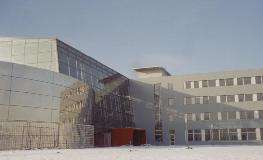
\includegraphics{bilder/garching.jpg}
	\caption{Bild der Mathe und Info Gebäudes in Garching b. München}
	\label{fig:garching}
\end{figure}

Als Beispiel kommen die Worte Grundlagen und Einleitung in den Index \index{Grundlagen} \index{Einleitung}

%%%%%%%%%%%%%%%%%%%%%%%%%%%%%%%%%%%%%%%%%%%%%%%%%%%%%%%%%%%%%%%%%%%%%%%%%%%%%%%
% *** Gleichungen ***
%%%%%%%%%%%%%%%%%%%%%%%%%%%%%%%%%%%%%%%%%%%%%%%%%%%%%%%%%%%%%%%%%%%%%%%%%%%%%%%
%
\section{Gleichungen}\label{sec:gleichungen}
%
Dies ist eine einfache Gleichung
%
\begin{eqnarray}\label{gl:einfache_gleichung}
  y & = & ax^2 + bx + c
\end{eqnarray}



\section{Quellcode}
Man kann mit \LaTeX{} super Quelltext oder Snippets setzen. Dazu muss man die Sprache konfigurieren und wie man möchte, dass der Quellcode aussieht. Das kann pro Snippet passieren. . 
\lstset{
	numbers=left, numberstyle=\tiny, numbersep=5pt,
basicstyle=\small, % print whole listing small 
%keywordstyle=\ttb\color{deepblue}
%identifierstyle=, % nothing happens 
%commentstyle=\color{white}, % white comments 
%stringstyle=\ttfamily, % typewriter type for strings 
%showstringspaces=false} % no special string spaces
}
\begin{lstlisting}[columns=fullflexible,showspaces=false,showtabs=false, language=Python, frame=single, caption={Fakultaetsberechnung}]
def factorial(num): 
  if num < 0: 
      print("Factorial of negative num does not exist")
  elif num == 0: 
    return 1
  else: 
  fact = 1
  while(num > 1): 
    fact *= num 
    num -= 1
  return fact 
\end{lstlisting}

\section{Tabellen}
Tabellen sind ebenfalls gleitende Objekte so wie Bilder. 
\begin{table}
	\centering
	\begin{tabular}{c|c}
		\textbf{Spalte 1} & \textbf{Spalte 2} \\
		\hline
		\hline
		Eintrag & Eintrag \\
		\hline
	\end{tabular}
	\caption{Eine Tabelle}
\end{table}

%%weitere Dateien hier einfgen um das Dokument zu partitionieren
% Sinnvoll ist nach Grundlagen und Methoden, z.b.
% Hardware \& Software
% Ergebnisse
% Zusammenfassung
		
%%%%Verzeichnisse, Bibliographie

%----------------------Abbildungs-, Tabellen-, und Listingsverzeichnis-----%
\listoffigures
\listoftables
%\listofalgorithms											
\lstlistoflistings
%\addcontentsline{toc}{chapter}{\numberline {Listings}}
\addchap{Abkürzungsverzeichnis}

%\chapter*{Abkürzungsverzeichnis}
\begin{acronym}[ECU]
	\acro{$s$}{Weg, physikalische Einheit}
\acro{$O(n)$}{Komplexität}
	\acro{ecu}[ECU]{Electronic Computing Unit}
	\acro{ETTI}{Elektrotechnik und Technische Informatik}
	\acro{eu}[EU]{Europäische Union}

	\acro{IoT}{Internet of Things}
\end{acronym}

%---------------------Literatur--------------------------
\printbibliography
							% alle Verzeichnisse

%%%%%%-------Anhang
%\include{anhang}														% eventuell einen Anhang	

\printindex																	% Index hier hin drucken
\end{document}
%----------Ende des Dokuments-------------------%